\documentclass[a4paper, 11pt]{article}


\usepackage[czech]{babel}
\usepackage{graphicx}
\usepackage[utf8]{inputenc}
\usepackage[left=3cm, top=4cm, text={15cm, 23cm}]{geometry}
\usepackage{times}
\usepackage{graphicx}
\usepackage[hyphens]{url}
\usepackage[unicode, colorlinks, hypertexnames=false]{hyperref}
\usepackage[czech, boxed]{algorithm2e}
\usepackage[perpage]{footmisc}
\usepackage{indentfirst}
\usepackage{algpseudocode}
\hypersetup{
    colorlinks=true,
    linkcolor=black,
    urlcolor=black,
}

\begin{document}
	%%%%%%%%%%%%%%%%%%%%%%%%%%%%%%%% Title page %%%%%%%%%%%%%%%%%%%%%%%%%%%
	\begin{titlepage}
		\begin{center}
			
\includegraphics[width=0.8 \linewidth]{FIT_logo.pdf}

			\vspace{\stretch{0.382}}

			\Huge{Simulační studie} \\
			\LARGE{\textbf{8: Vojenské simulátory}}

			\vspace{\stretch{0.618}}
		\end{center}

		\begin{minipage}{0.5 \textwidth}
			\Large
			3. 12. 2022
		\end{minipage}
		\hfill
		\begin{minipage}[r]{0.5 \textwidth}
			\Large
			\begin{tabular}{ll}
			    Martin Zmitko & (xzmitk01)
			\end{tabular}
		\end{minipage}
	\end{titlepage}
	\clearpage

	%%%%%%%%%%%%%%%%%%%%%%%%%%%%%%%% Contents %%%%%%%%%%%%%%%%%%%%%%%%%%%%%%%%%%%%%
	\pagenumbering{arabic}
	\setcounter{page}{1}
	\tableofcontents
	\clearpage

	%%%%%%%%%%%%%%%%%%%%%%%%%%%%%%%% 1. Introduction %%%%%%%%%%%%%%%%%%%%%%%%%%%%%%%%%%%%%%

	\section{Úvod}
    Tato práce do předmětu IMS se věnuje vojenské simulaci. Cílem bylo provést simulaci aktivního bojiště a zaměřit se na chování vojáků, především na délku bitev a ztrátách na životech, při změnách aktuálních podmínek na bojišti. Tyto informace jsou klíčové pro světové armády, umožňují lepší logistické plánování zásobování a dávají lepší pohled na potřebné vybavení vojáků.

	\subsection{Zdroje faktů}
    K získání informací byly použity internetové zdroje. Vzhledem k povaze tématu ale nebylo možné získat všechny potřebné parametry modelu, jednak kvůli utajení informací ze strany vlád zemí, bojiště je ale také chaotické místo, kde se konkrétní informace o chování vojáků stěží sbírají. Důležitou součástí simulace je také lidské chování, které je často náhodné a nevyzpytatelné.

	%%%%%%%%%%%%%%%% 2. Facts %%%%%%%%%%%%%%%
	\section{Fakta}
    Pro vytvoření modelu byla použita následující fakta:
    \begin{itemize}
        \item průměrná rychlost pohybu vojáka v ideálních podmínkách je $1.5\ ms^{-1}$, při běhu $3\ ms^{-1}$ \cite{speed}
        \item člověk je pouhým okem schopen rozeznat dalšího člověka na vzdálenost až 500~m, spolehlivě ho rozpoznat na 250~m \cite{vision}
        \item maximální dosah pušek ráže 5.56 mm je 300 m, spolehlivý dosah je méně než 100 m \cite{guns}
    \end{itemize}

	%%%%%%%%%%%%%%%%%%%%%%%%%%%%%%%% 3. Concept of model %%%%%%%%%%%%%%%%%%%%%%%%%%%
	\section{Koncepce modelu}
    Model je řešen pomocí multi-agentní simulace. Na bojišti s rozměry 1000 m x 1000 m jsou umístěni vždy na stejných místech vojáci -- agenty simulace. Na bojišti panují ve výchozím stavu ideální podmínky -- terén je snadno průchodný, nic neomezuje viditelnost, bojiště je ploché. Bojují proti sobě dvě strany -- jedna strana brání svou základnu a její vojáci v simulaci začínají v její blízkosti, druhá se ji snaží dobýt a vojáci začínají na druhé straně bojiště. Na obou stranách bojuje 20 vojáků.

    Každý voják je vybaven puškou ráže 5.56 mm, munice v modelu omezená není. Vojákovy fyziologické potřeby taktéž nejsou v modelu zahrnuty. Každý voják je určen pomocí unikátního identifikátoru, příslušností k jedné ze stran a souřadnicemi, na kterých se nachází.

    Chování vojáka je následující (rozhodování probíhá v tomto pořadí, voják vždy provede jen jednu akci):

    Voják je v základně:
    \begin{itemize}
        \item pokud základnu brání a nejsou v ní žádní útočníci, základnu opouští
        \item pokud jsou v základně vojáci druhého týmu, s pravděpodobností 5\% jednoho eliminuje
    \end{itemize}
   Voják není v základně:
    \begin{itemize}
        \item pokud je voják vzdálený méně než 10 m od základny:
        \begin{itemize}
            \item pokud je útočník, vstoupí do základny
            \item pokud je obránce, vstoupí do základny, pokud se v ní nachází útočníci
        \end{itemize}
        \item pokud je obránce a v základně jsou útočníci, s pravděpodobností podle vztahu \\ $1 - e^{-0.05 * count(utocnici)}$ se vydá směrem k základně, určeným normálním rozdělením se středem přímý úhel k základně a směrodatnou odchylkou $0.1\pi$ a urazí vzdálenost určenou normálním rozdělením se středem 30 m a směrodatnou odchylkou 2 m
        \item voják prohledá okolí a spatří nepřátele s pravděpodobností podle vztahu $e^{-0.01 * vzdalenost}$
        \item pokud spatří nepřítele, po nejbližším vystřelí. Zasáhne ho s pravděpodobností \\ $e^{-0.005 * vzdalenost}$
        \item pokud nepřítele nespatří, pohne se následovně:
        \begin{itemize}
            \item pokud je útočník, pohne se směrem daným normálním rozdělením se středem přímý úhel k základně a směrodatnou odchylkou $0.3\pi$ a urazí vzdálenost danou normálním rozdělením se středem 15 m a směrodatnou odchylkou 2 m
            \item pokud je obránce, pohne se směrem daným normálním rozdělením se středem přímý úhel k základně a směrodatnou odchylkou $0.3\pi$ a urazí vzdálenost danou normálním rozdělením se středem daným vztahem $\frac{(vzdalenost\_zakladny - 50)^3}{1000}$, omezeným v intervalu $\langle -40, 40 \rangle$ a směrodatnou odchylkou 2 m
        \end{itemize}
    \end{itemize}

    Simulace probíhá v krocích, přičemž každý krok zabere 10 s reálného času. V každém kroku se provede aktualizace každého vojáka naráz. Simulace končí buď zabráním základny druhou stranou (celkem musí nepřátelští vojáci strávit v základně 100 kroků, pokud je v základně vojáků víc, strávený čas se sčítá), po eliminaci všech vojáků v jednom týmu, nebo po uplynutí 24 hodin (8640 kroků).

	%%%%%%%%%%%%%%%%%%% 4. Implementation %%%%%%%%%%%%%%%%%%%%%%%%
	\section{Implementace}
	Simulace byla napsána v jazyce C++, standard C++17, byl použit kompilátor g++. Každý voják je implementován třídou \texttt{Agent}. Tato třída obsahuje všechny informace o agentovi, také implementuje všechny metody potřebné pro simulaci -- pohyb, střelba, výpočet vzdáleností a úhlů k základně a ostatním vojákům.

    Ke grafické vizualizaci je použita knihovna SFML, knihovna je přibalena ke zdrojovému kódu. Projekt se přeloží pomocí přiloženého Makefile příkazem \texttt{make} a spustí příkazem \texttt{make run}.\\ \textbf{K běhu programu je nutná možnost grafického výstupu.}

	%%%%%%%%%%%%%%% 5. Experiments %%%%%%%%%%%
	\section{Experimenty}
	Výsledky simulace pro výchozí parametry -- tedy při ideálních podmínkách na bojišti ukazují, že se bitvy odehrají relativně rychle, kolem 10 minut. Bitva končí vždy eliminací jednoho z týmů a šance na vítězství mají obě strany podobné. Odkaz na video zachycující vizualizaci simulace: \url{https://www.youtube.com/watch?v=RaRb-46AlYQ} \newpage
    \begin{figure}[h]
        \centering
        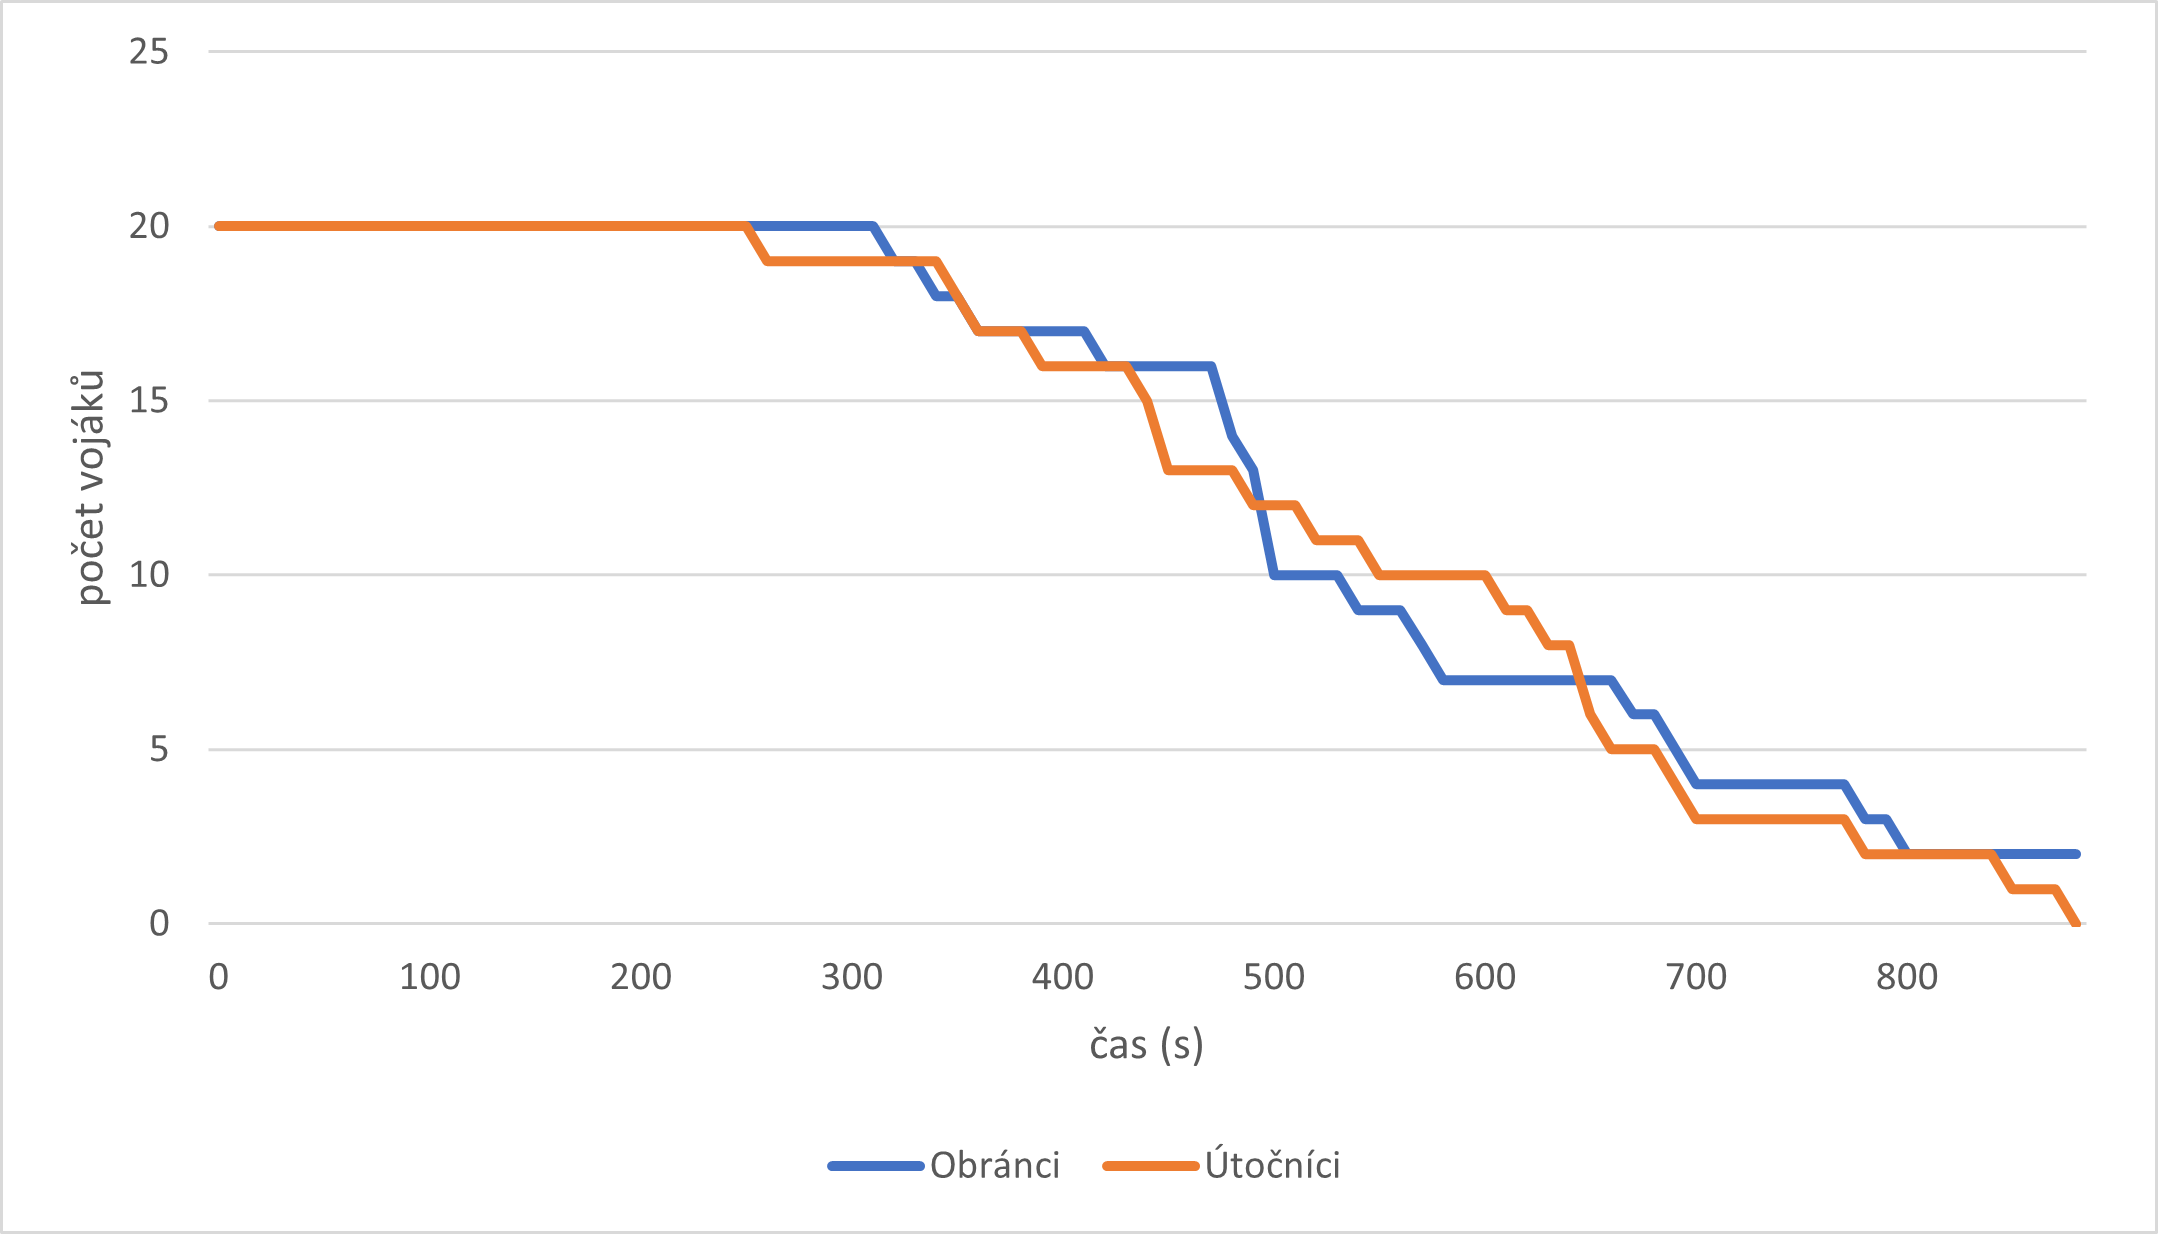
\includegraphics[width=0.8\textwidth]{graph1.png}
        \caption{Graf počtu vojáků v čase, ideální podmínky (výhra obránců eliminací útočníků)}
    \end{figure}

    \subsection{Experiment 1}
    Cílem tohoto experimentu je ověřit vývoj bitvy při snížených podmínkách -- v tomto případě mlha s maximální viditelností 100 m. Upravíme proto vztah pravděpodobnosti spatření protivníka na $e^{-0.03 * vzdalenost}$.
    \begin{figure}[h]
        \centering
        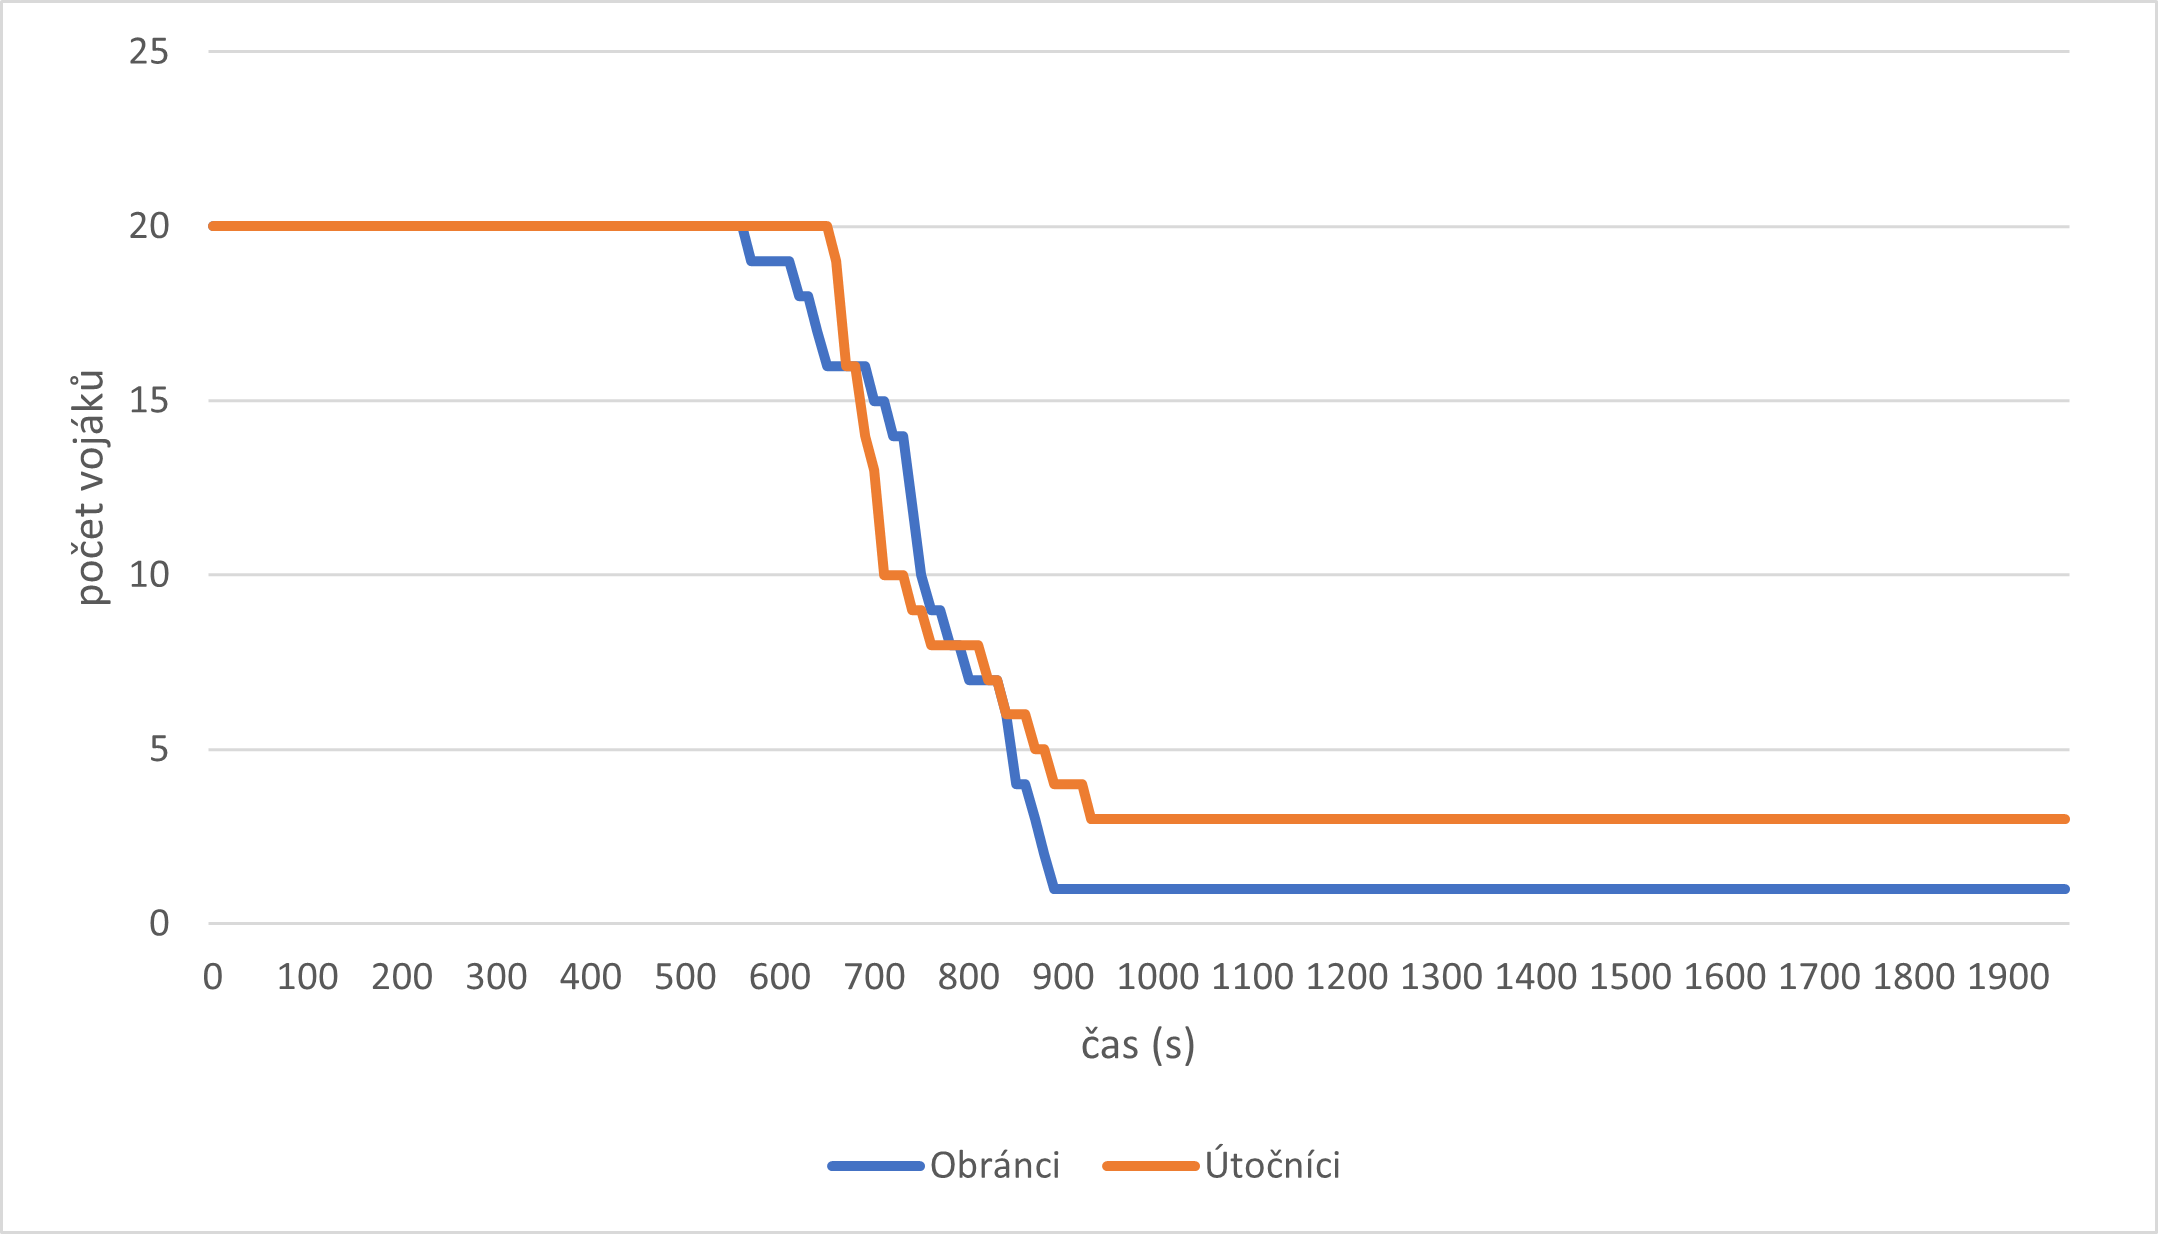
\includegraphics[width=0.8\textwidth]{graph2.png}
        \caption{Graf počtu vojáků v čase, viditelnost 100 m (výhra útočníků zabráním základny)}
    \end{figure}

    Doba bitvy se oproti ideálním podmínkám prodloužila v průměru o 50 \% a asi v polovině případů se útočníkům povedlo infiltrovat základnu. Boj v základně byl vyrovnaný a obě strany vyhrávaly se stejnou úspěšností. Konflikt byl ale ostřejší, většina úmrtí nastala v krátkém časovém úseku.

    \subsection{Experiment 2}
    Cílem tohoto experimentu je ověřit vývoj bitvy při téměř nulové viditelnosti. Vztah pro výpočet pravděpodobnosti spatření byl tedy upraven na $e^{-0.3 * vzdalenost}$.
    \begin{figure}[h]
        \centering
        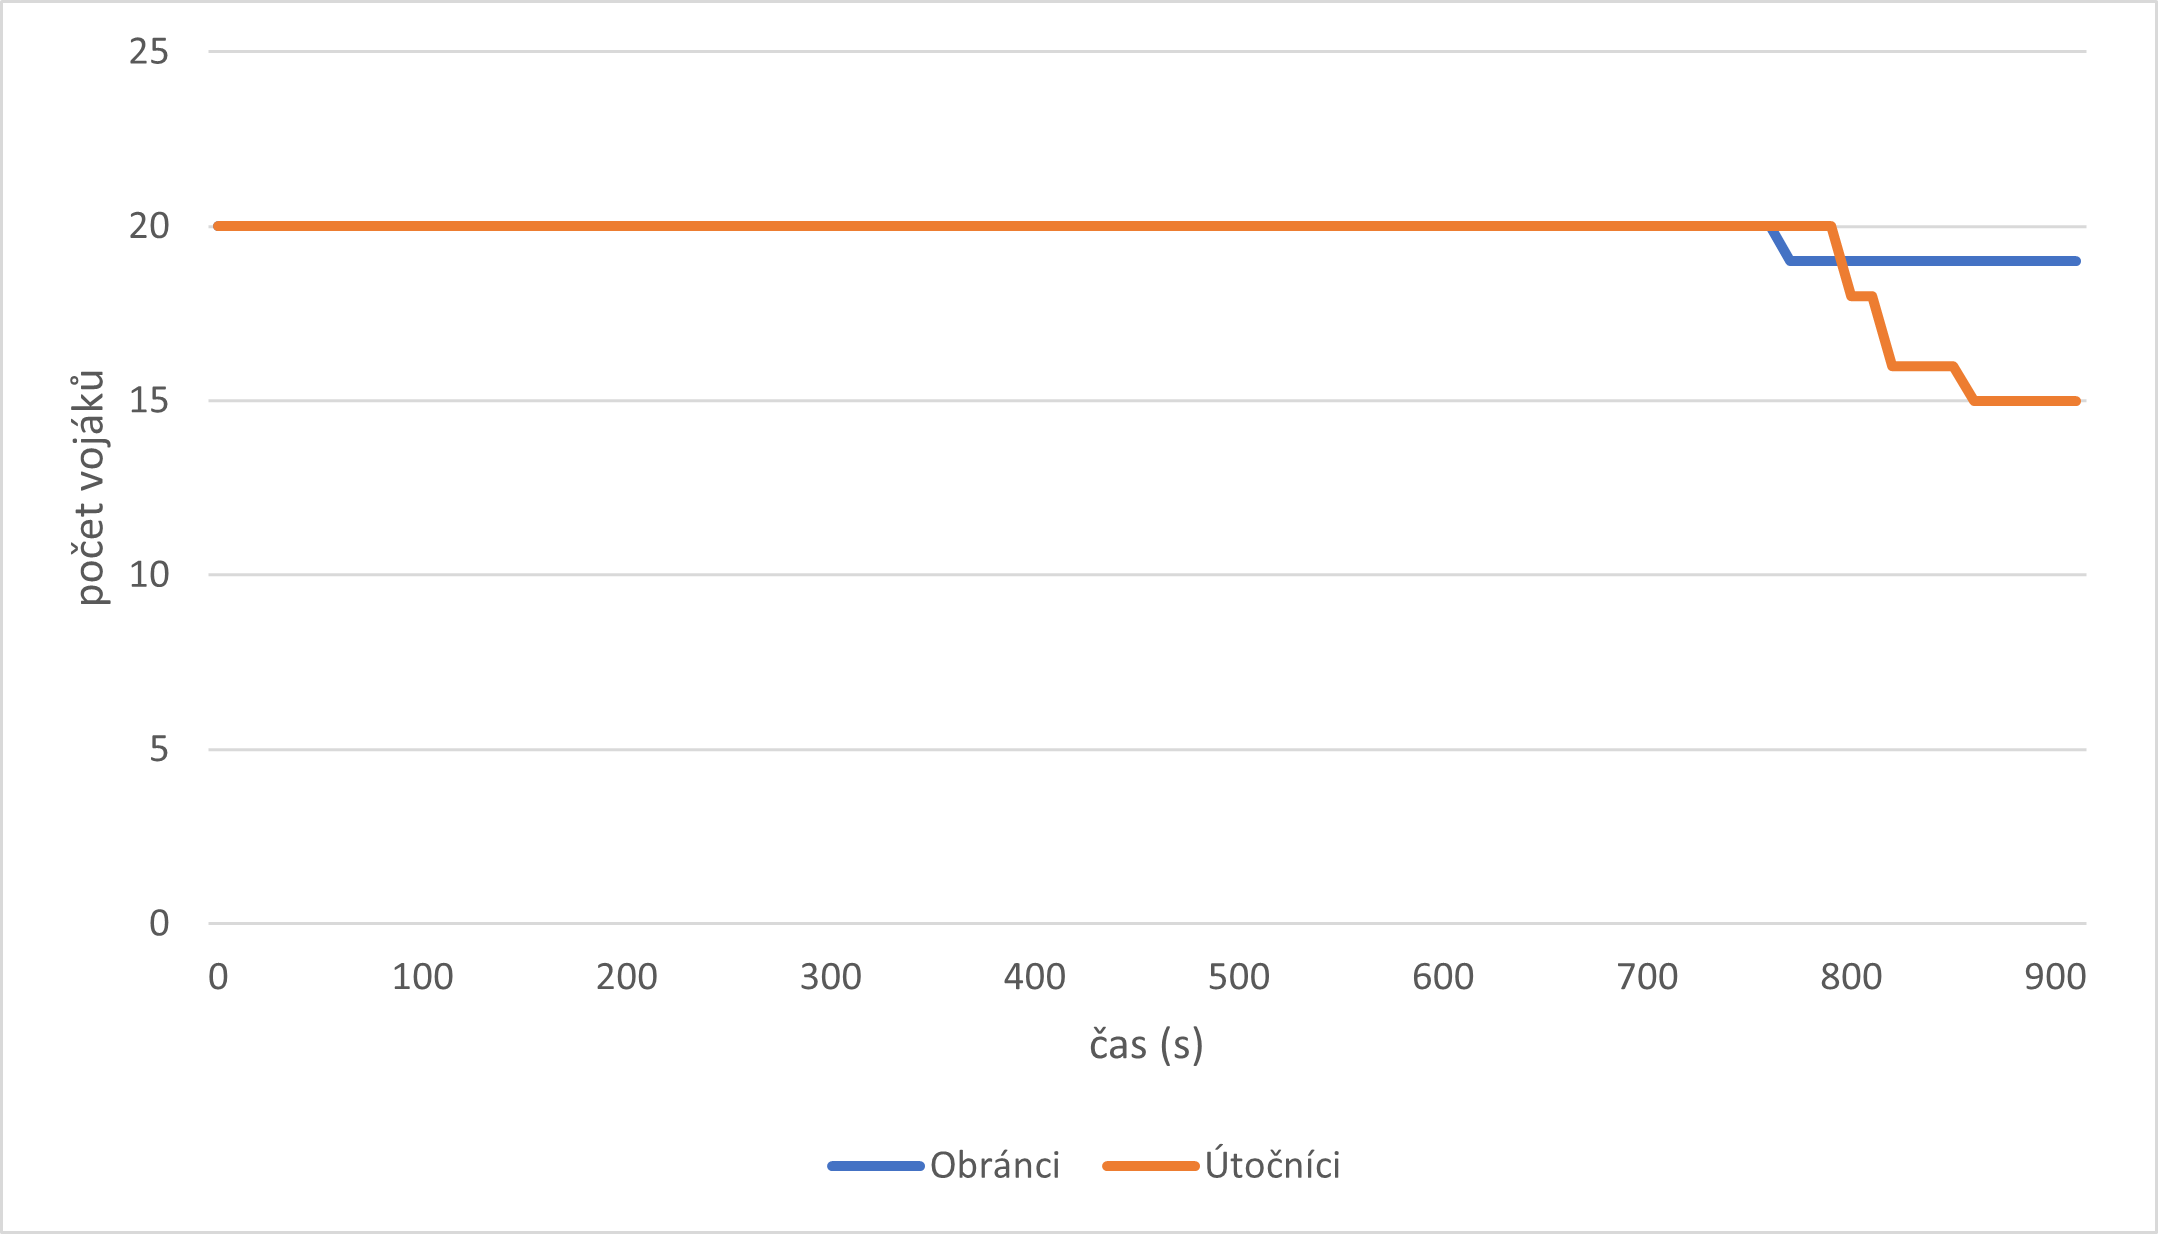
\includegraphics[width=0.8\textwidth]{graph3.png}
        \caption{Graf počtu vojáků v čase, viditelnost méně než 10 m (výhra útočníků zabráním základny)}
    \end{figure}

    V těchto podmínkách se bitva transformovala -- vojáci neměli šanci se navzájem na bojišti spatřit a každá bitva skončila zabráním základny útočníky. Délka bitev byla podobná, jako v ideálních podmínkách, vojáci neztráceli čas střelbou, ale útočili rovnou na základnu.

    \subsection{Experiment 3}
    V tomto experimentu zjišťuji vliv hůře prostupného terénu (např. v mokřadu) na trvání a podobu bitvy. Nová průměrná rychlost vojáka bude nyní $0.3\ ms^{-1}$, vzdálenost uražená vojákem v jednom kroku se tedy změní na normální rozdělení se středem 3 m a směrodatnou odchylkou 0.5 m.
	\begin{figure}[h]
        \centering
        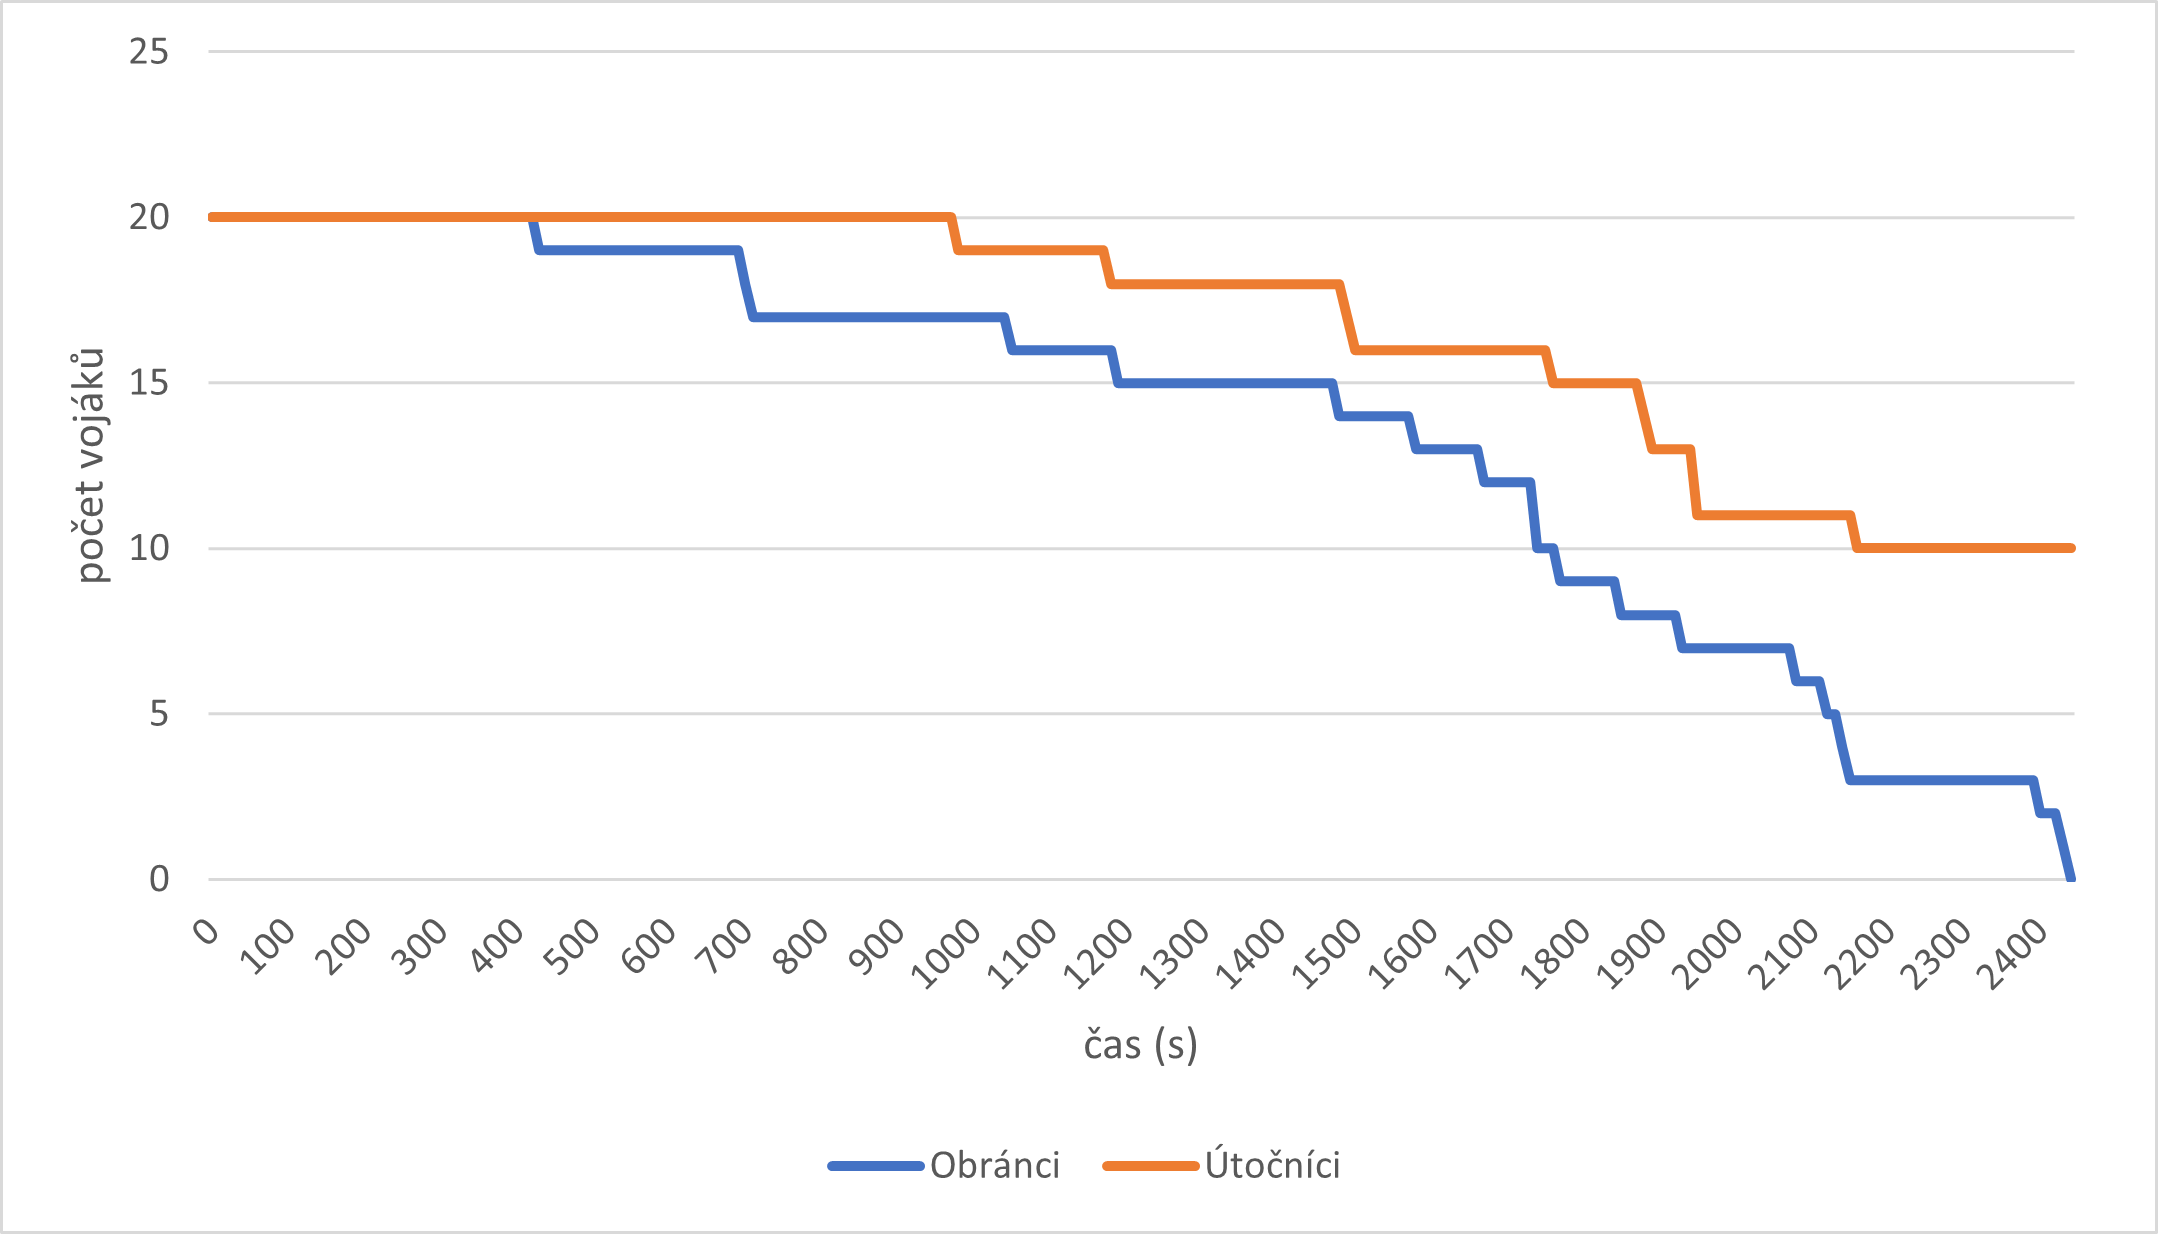
\includegraphics[width=0.8\textwidth]{graph4.png}
        \caption{Graf počtu vojáků v čase, zhoršená prostupnost terénu (výhra útočníků eliminací obránců)}
    \end{figure}

    Bylo zjištěno, že zhoršená prostupnost terénu zásadně ovlivní délku bitvy -- v tomto případě o 300 \%. Změnil se i charakter bitvy -- útočníci nemají šanci se dostat k základně a bitva končí postupnou eliminací jednoho z týmů.

	%%%%%%%%%%%%%%%%% Summary of simulation experiments and conclusion %%%%%%%%%%%%%%%%%%
	\section{Závěr}
    Bylo zjištěno, že změna podmínek na bojišti má zásadní vliv na vývoj a výsledek bitvy. Z naměřených dat plyne, že je velmi důležité sledovat podmínky na bojišti a zásobit vojáky dostatkem jídla a tekutin, protože podmínky bojiště mají zásadní vliv na trvání bitvy.
 
	%%%%%%%%%%%%%%%%% Bibliography %%%%%%%%%%%%%%%%%%
	\clearpage
	\nocite{*}
	\renewcommand{\refname}{Zdroje}
	\bibliography{bibliography.bib}
	\bibliographystyle{czechiso.bst}
\end{document}